\chapter[Resultados Preliminares]{Resultados Preliminares}
\label{sec:Resultados}

Para validar o sistema proposto, foram realizados testes no ambiente virtual \textit{PureData}, focando na filtragem controlada por um botão central e no funcionamento dos efeitos, incluindo o controle automático do volume e a configuração dos parâmetros de cada efeito.

\section{Resultados de Filtragem}

Nesta seção, são apresentados os resultados de ensaios realizados no ambiente virtual \textit{PureData}, simulando a filtragem em diferentes frequências de corte.

Utilizaram-se duas músicas: \cite{track01} e \cite{track02}, das quais foram selecionadas janelas de dois segundos. A escolha desse intervalo considerou a presença de elementos de todas as bandas de frequência. A filtragem foi realizada usando filtros passa-altas com as seguintes frequências de corte:

\begin{itemize}
    \item 0 Hz
    \item 20 Hz
    \item 300 Hz
    \item 4 kHz
    \item 22 kHz
\end{itemize}

Para cada frequência de corte, foram obtidas as representações do sinal tanto no domínio do tempo quanto no domínio da frequência, utilizando a Transformada de Fourier de Curto Prazo (STFT - \textit{Short Time Fourier Transform}). As figuras a seguir mostram as representações em função da frequência de corte para ambas as músicas de referência.

Na Figura \ref{fig40}, é mostrada a janela do arquivo de áudio no domínio do tempo, evidenciando a presença de \textit{kicks} e elementos de maiores frequências.

\begin{figure}[h]
    \centering
    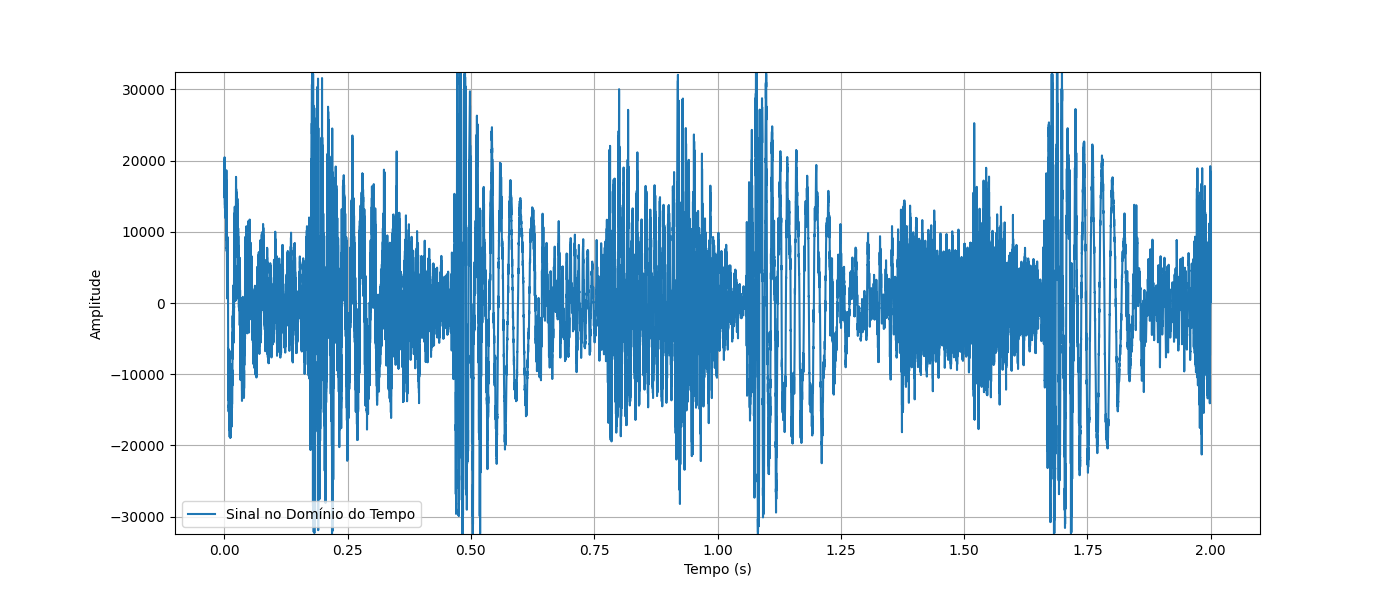
\includegraphics[width=0.8\textwidth]{figuras/fig40.png}
    \caption{música 1 no domínio do tempo sem filtragem}
    \label{fig40}
\end{figure}

Na Figura \ref{fig41}, a STFT da mesma janela revela uma maior presença de elementos em baixa frequência. Assim como na Figura \ref{fig40}, é possível observar a variação de elementos agudos ao longo da música.

\begin{figure}[h]
    \centering
    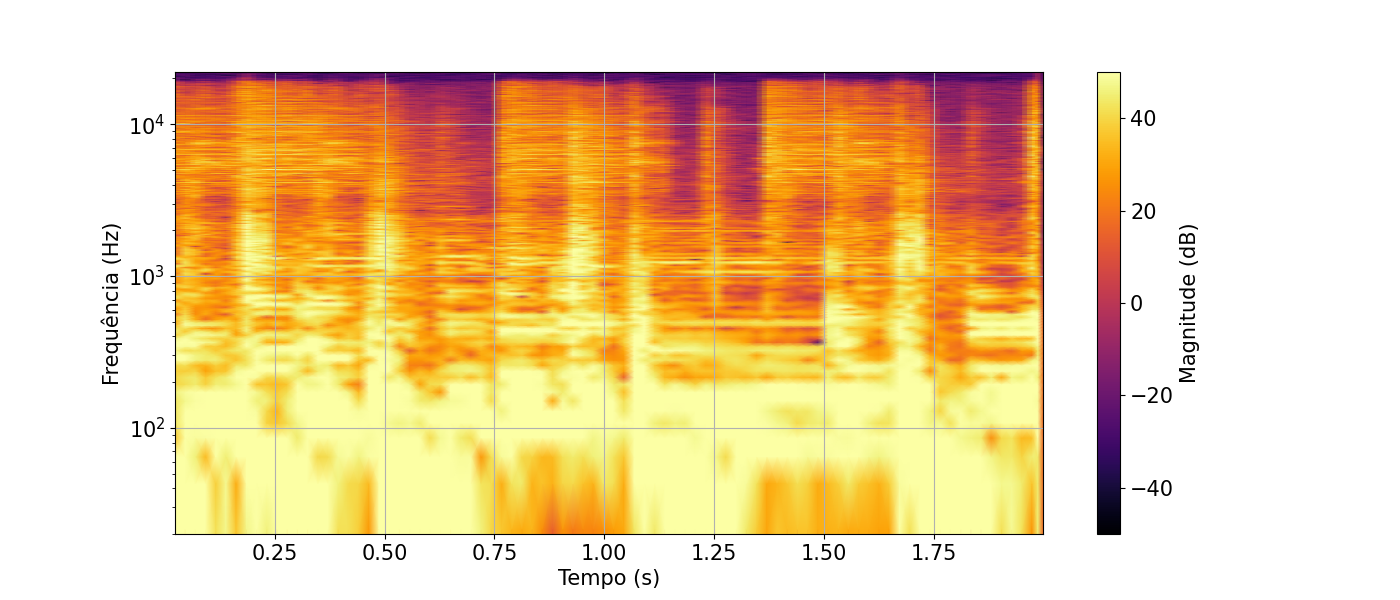
\includegraphics[width=0.8\textwidth]{figuras/fig41.png}
    \caption{música 1 no domínio da frequência sem filtragem}
    \label{fig41}
\end{figure}

Após a aplicação de um filtro passa-altas com frequência de corte de 20 Hz, as alterações no sinal são sutis. A Figura \ref{fig24} mostra o sinal no domínio do tempo com a filtragem aplicada.

\begin{figure}[h]
    \centering
    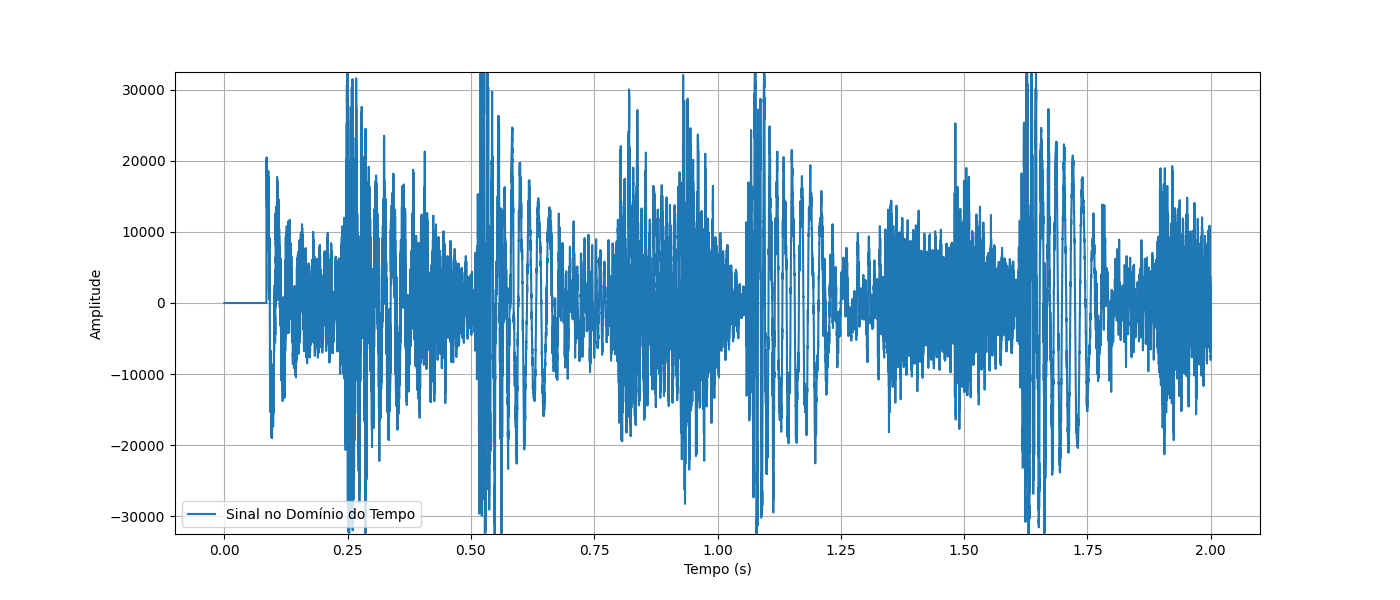
\includegraphics[width=0.8\textwidth]{figuras/fig24.png}
    \caption{música 1 no domínio do tempo com frequência de corte de 20 Hz}
    \label{fig24}
\end{figure}

A análise da Figura \ref{fig25} confirma que as componentes em frequência não sofreram grandes alterações após a aplicação do filtro passa-altas com frequência de corte de 20 Hz.

\begin{figure}[h]
    \centering
    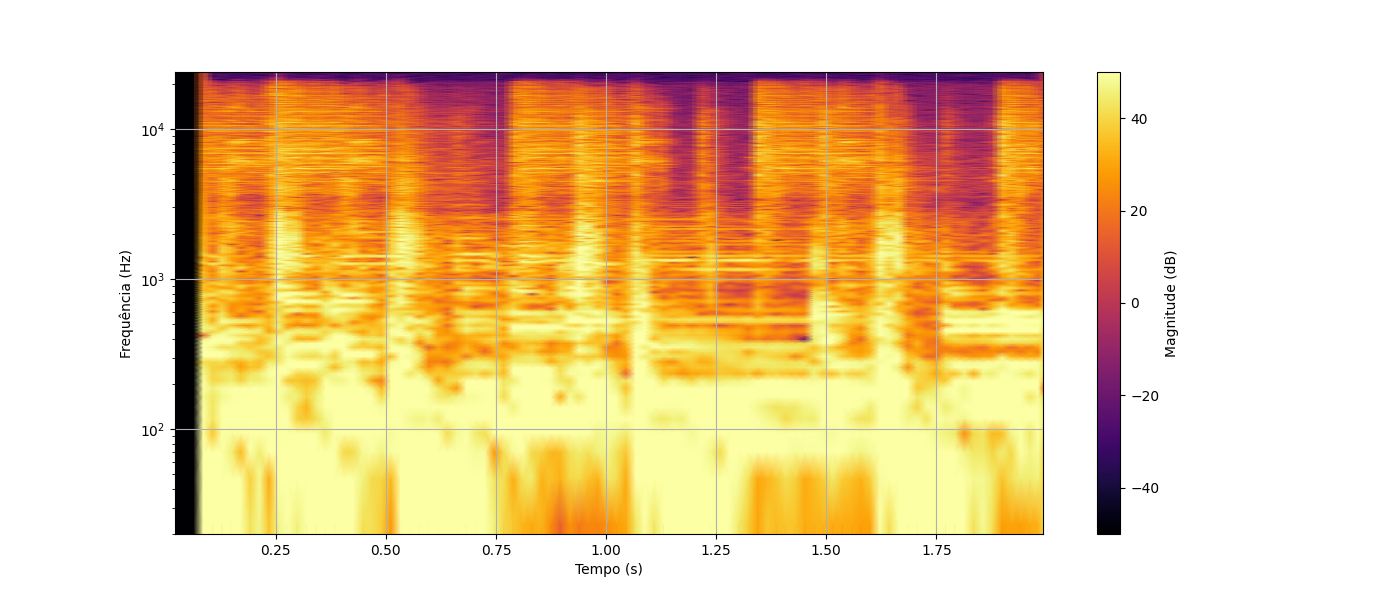
\includegraphics[width=0.8\textwidth]{figuras/fig25.png}
    \caption{música 1 no domínio da frequência com frequência de corte de 20 Hz}
    \label{fig25}
\end{figure}


Em \textit{mixers} convencionais, o botão correspondente às baixas frequências geralmente controla a banda de 300 Hz. Portanto, no presente estudo, o controle de frequência foi ajustado para aproximar a frequência de corte de 300 Hz.

Os resultados dessa filtragem podem ser visualizados nas Figuras \ref{fig28} e \ref{fig29}. A Figura \ref{fig28} mostra que houve uma atenuação significativa dos sinais, evidenciada pelos valores máximos da amplitude. Observa-se também a ausência de sinais de baixa frequência, que estavam presentes como envelopes nos sinais não filtrados.

\begin{figure}[h]
    \centering
    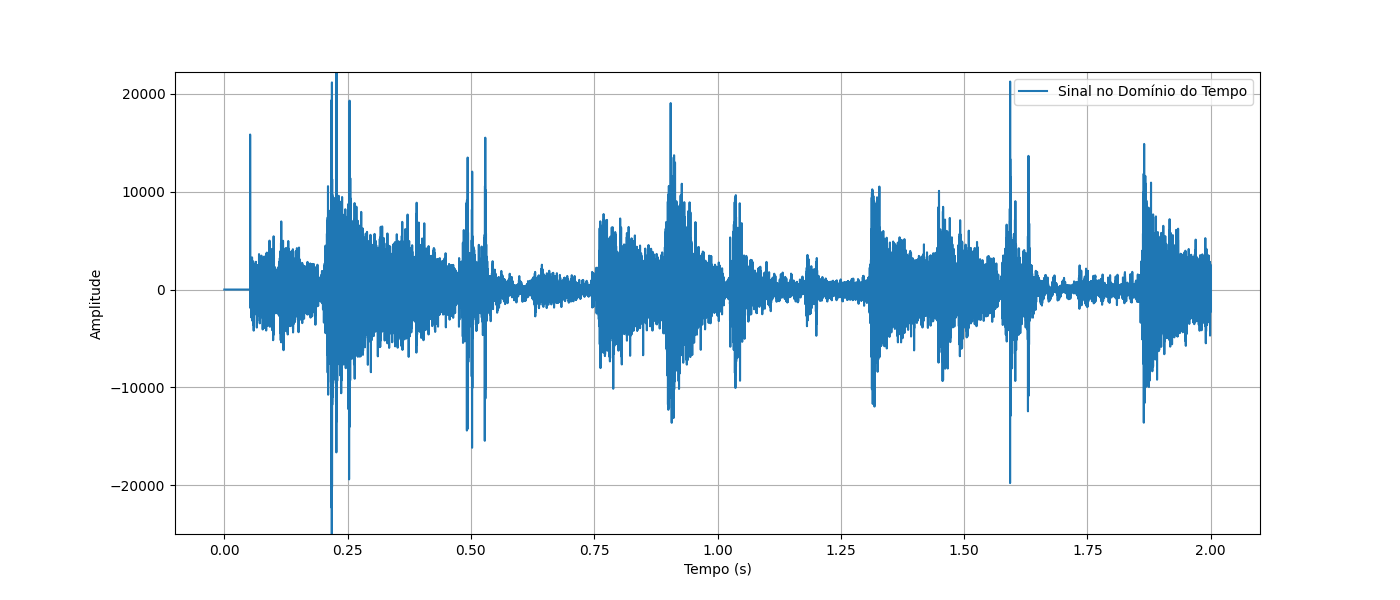
\includegraphics[width=\textwidth]{figuras/fig28.png}
    \caption{música 1 no domínio do tempo com uma frequência de corte de 300 Hz}
    \label{fig28}
\end{figure}

A atenuação da banda de 300 Hz é confirmada na Figura \ref{fig29}, onde se observa uma redução de aproximadamente 30 dB nas componentes de baixa frequência.

\begin{figure}[h]
    \centering
    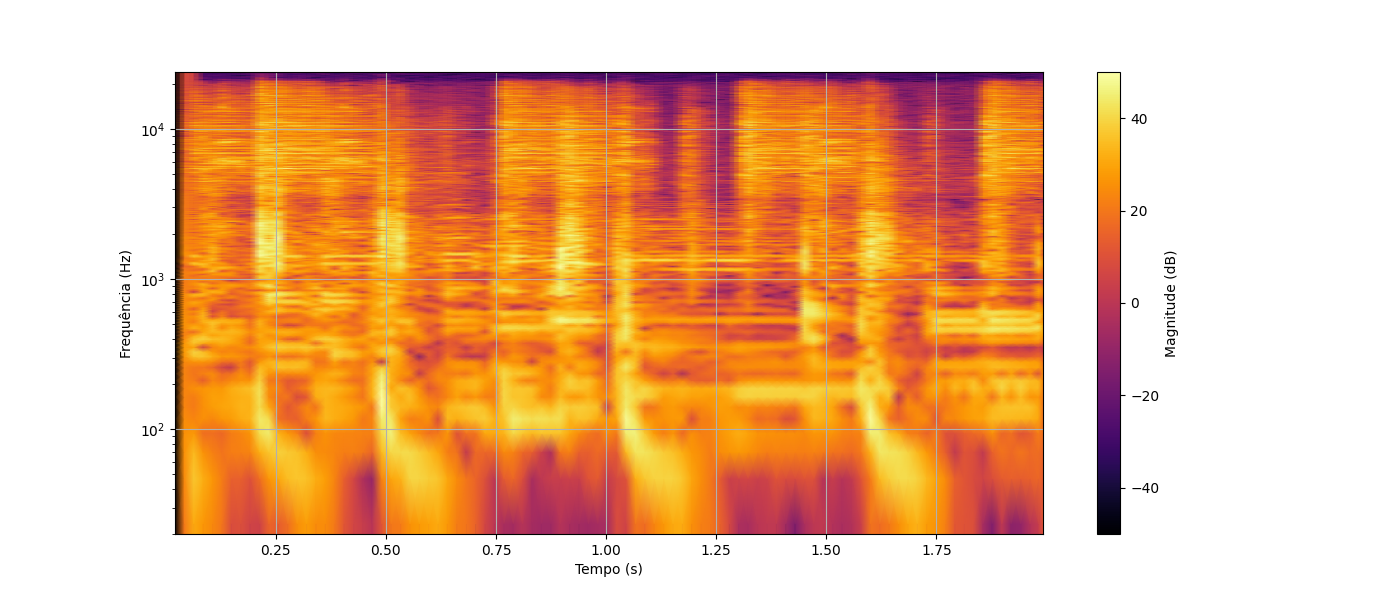
\includegraphics[width=0.8\textwidth]{figuras/fig29.png}
    \caption{música 1 no domínio da frequência com uma frequência de corte de 300 Hz}
    \label{fig29}
\end{figure}

A próxima frequência de corte utilizada foi de 4 kHz, que, conforme descrito no Capítulo \ref{cha:fundamentacao}, é onde se encontram os elementos médios. A Figura \ref{fig26} mostra a atenuação dos sinais em comparação com as filtragens anteriores.

\begin{figure}[h]
    \centering
    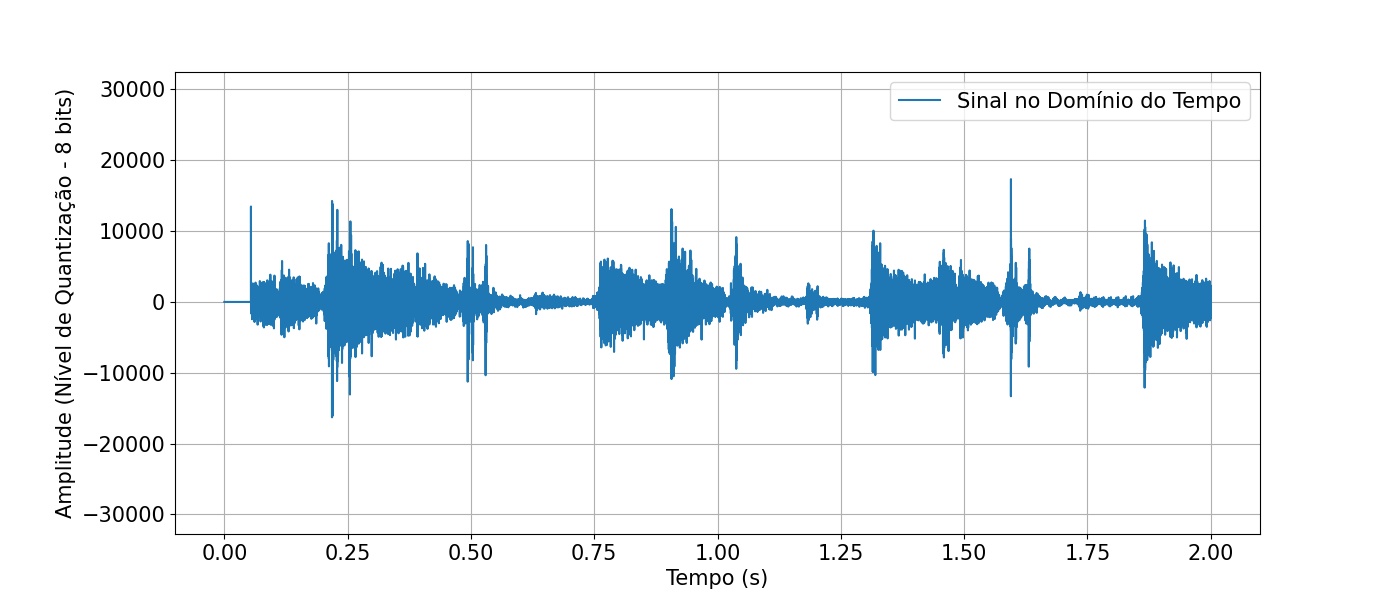
\includegraphics[width=0.8\textwidth]{figuras/fig26.png}
    \caption{música 1 no domínio do tempo com uma frequência de corte de 4 kHz}
    \label{fig26}
\end{figure}

Na Figura \ref{fig27}, que apresenta a STFT, observa-se uma atenuação significativa das componentes na banda de 4 kHz, com algumas componentes chegando a 0 dB em determinados pontos.

\begin{figure}[h]
    \centering
    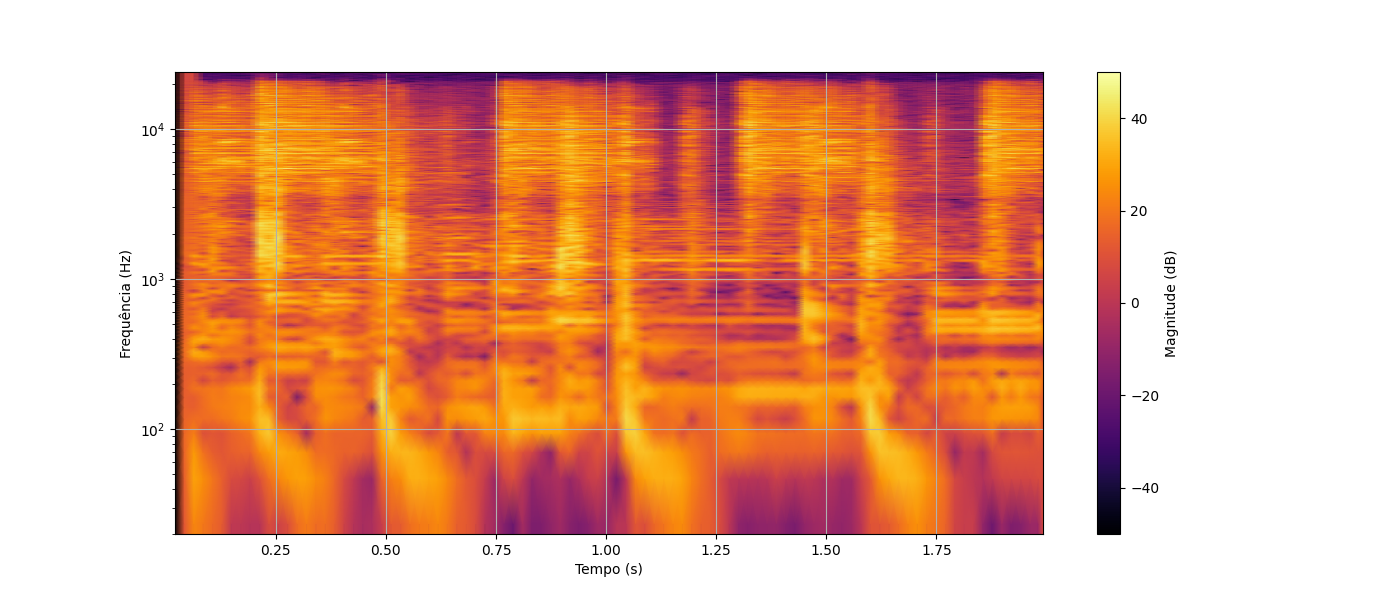
\includegraphics[width=0.8\textwidth]{figuras/fig27.png}
    \caption{música 1 no domínio da frequência com uma frequência de corte de 4 kHz}
    \label{fig27}
\end{figure}

Para a música \cite{track01}, uma análise final foi realizada utilizando uma frequência de corte de 24 kHz. Este ajuste visou atenuar os elementos restantes, considerados agudos ou brilhantes. A Figura \ref{fig30} mostra a atenuação das amplitudes dos sinais em comparação com as filtragens anteriores.

\begin{figure}[h]
    \centering
    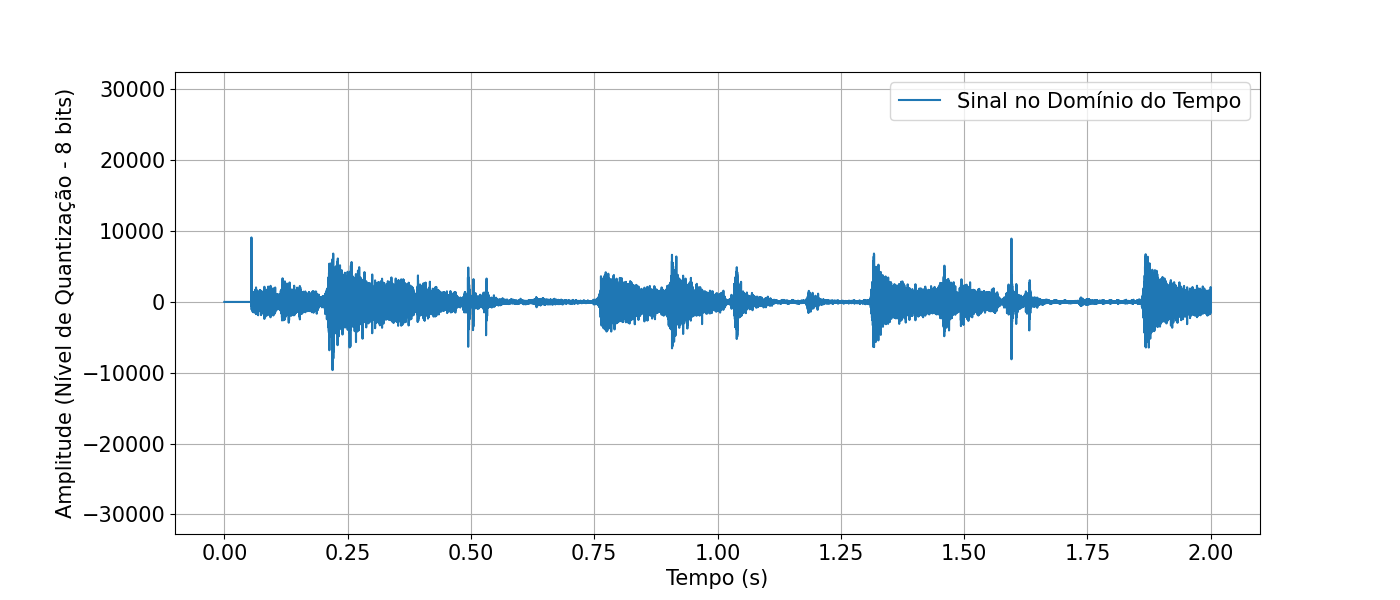
\includegraphics[width=0.8\textwidth]{figuras/fig30.png}
    \caption{música 1 no domínio do tempo com uma frequência de corte de 22 kHz}
    \label{fig30}
\end{figure}

Além disso, na Figura \ref{fig31}, observa-se a atenuação da banda correspondente, com elementos variando de 10 dB a -40 dB. Comparado com a STFT da filtragem anterior, nota-se uma atenuação generalizada do sinal.

\begin{figure}[h]
    \centering
    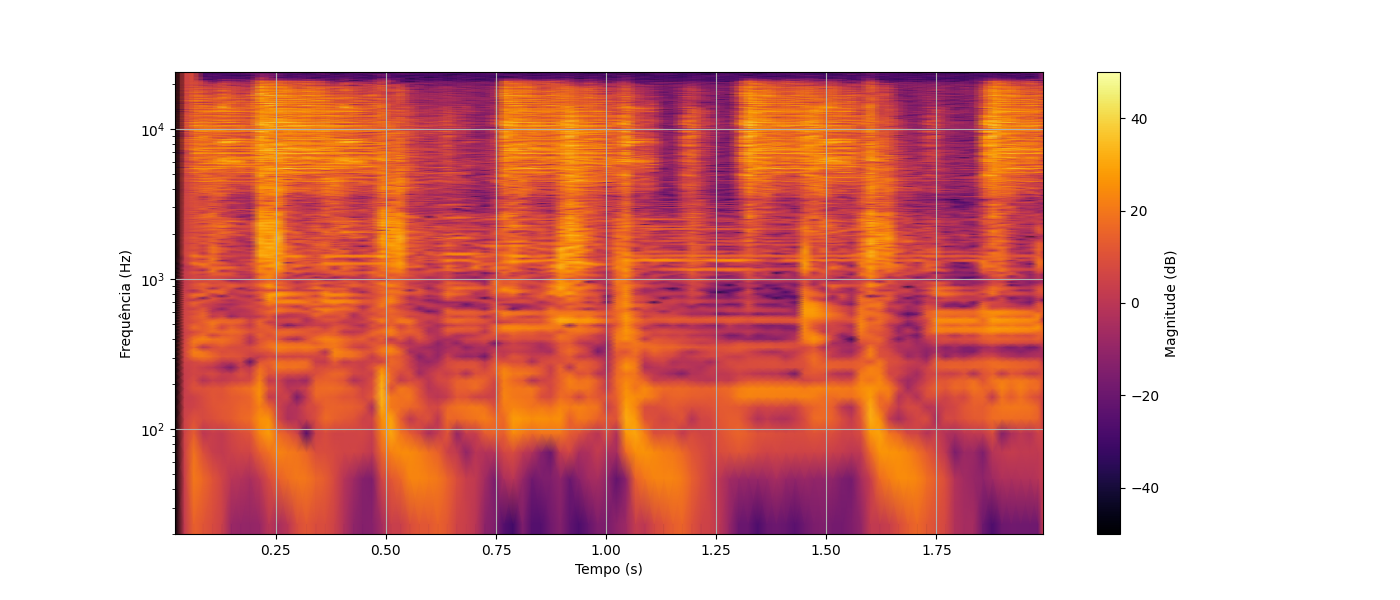
\includegraphics[width=0.8\textwidth]{figuras/fig31.png}
    \caption{música 1 no domínio da frequência com uma frequência de corte de 22 kHz}
    \label{fig31}
\end{figure}

A análise realizada na música \cite{track01} foi também aplicada à música \cite{track02}. Os resultados obtidos no domínio do tempo e da frequência, utilizando a STFT, foram semelhantes aos observados para a música \cite{track01}.

É importante notar que, conforme o botão de frequência de corte avança, a frequência de corte do filtro do canal 1 aumenta, atenuando primeiro as menores frequências e, em seguida, as maiores frequências. Em contraste, para o canal 2, a frequência de corte começa alta e diminui, ampliando as componentes de frequência do sinal da música \cite{track02}.

\section{Resultados de Efeitos}

Os efeitos são controlados pela frequência central, que determina o volume do efeito, e um botão de duas posições, que seleciona o efeito a ser utilizado. Testes foram realizados para verificar essas operações.

Primeiramente, simulou-se o volume do efeito em função da posição do botão central. Em seguida, foram realizadas simulações variando os parâmetros dos efeitos.

\subsection{Automação de Efeitos}

Para validar o controle automático do volume, isolou-se a saída dos efeitos e variaram-se as frequências, que geram diferentes volumes de efeitos. Os sinais no domínio do tempo foram analisados, conforme mostrado nas figuras abaixo.

\begin{figure}[h]
    \centering
    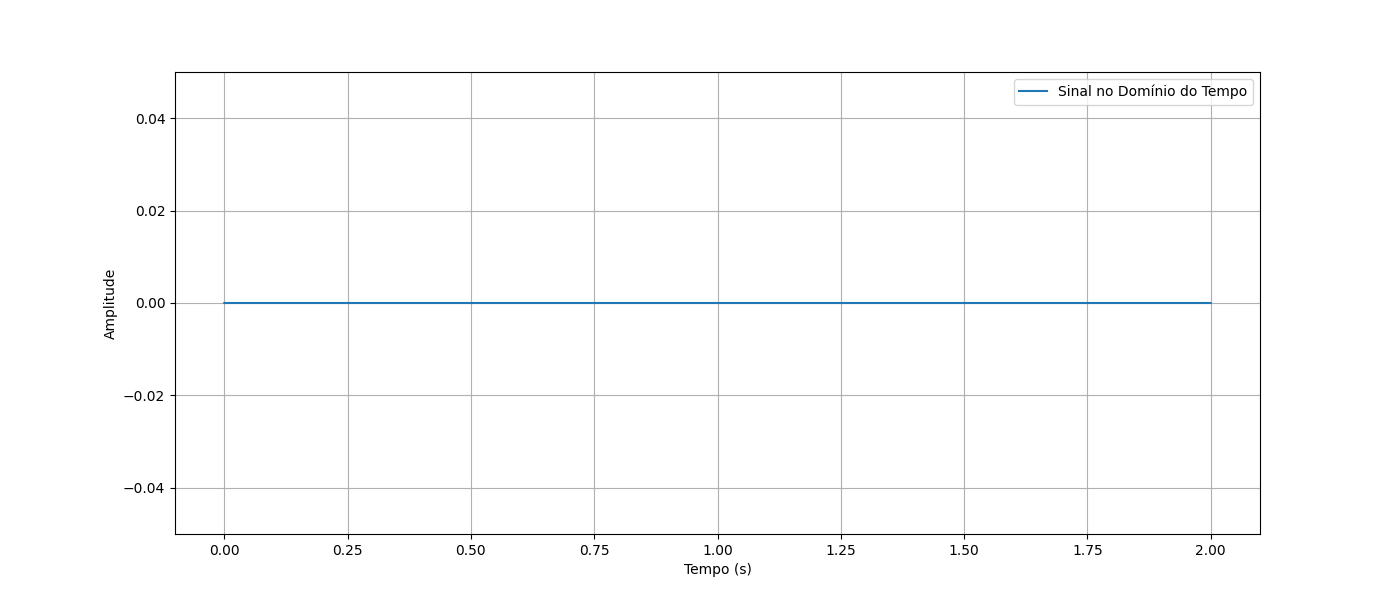
\includegraphics[width=0.8\textwidth]{figuras/fig66.png}
    \caption{canal de efeito \textit{reverb} isolado com música 1 a um volume nulo}
    \label{fig66}
\end{figure}

Na Figura \ref{fig66}, a frequência central utilizada foi a mínima. De acordo com a função mostrada na Figura \ref{fig49}, o volume esperado seria nulo. Assim, o sinal obtido também foi constante e nulo, como esperado.

\begin{figure}[h]
    \centering
    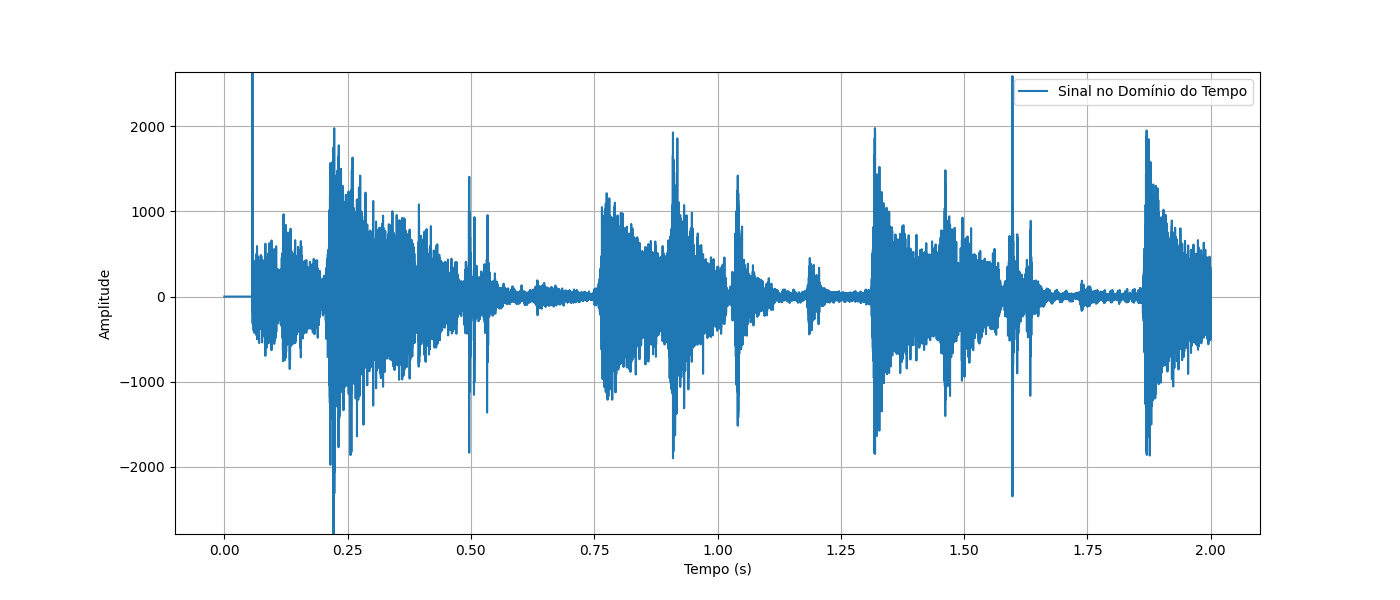
\includegraphics[width=0.8\textwidth]{figuras/fig67.png}
    \caption{canal de efeito \textit{reverb} isolado com música 1 a um volume de 0.3312}
    \label{fig67}
\end{figure}

Em seguida, variou-se a posição do botão central para atingir a frequência de 9454 Hz, resultando em um volume de 0.3312. A Figura \ref{fig67} mostra um sinal similar ao da música \cite{track01}, mas com uma amplitude específica.

\newpage

\begin{figure}[h]
    \centering
    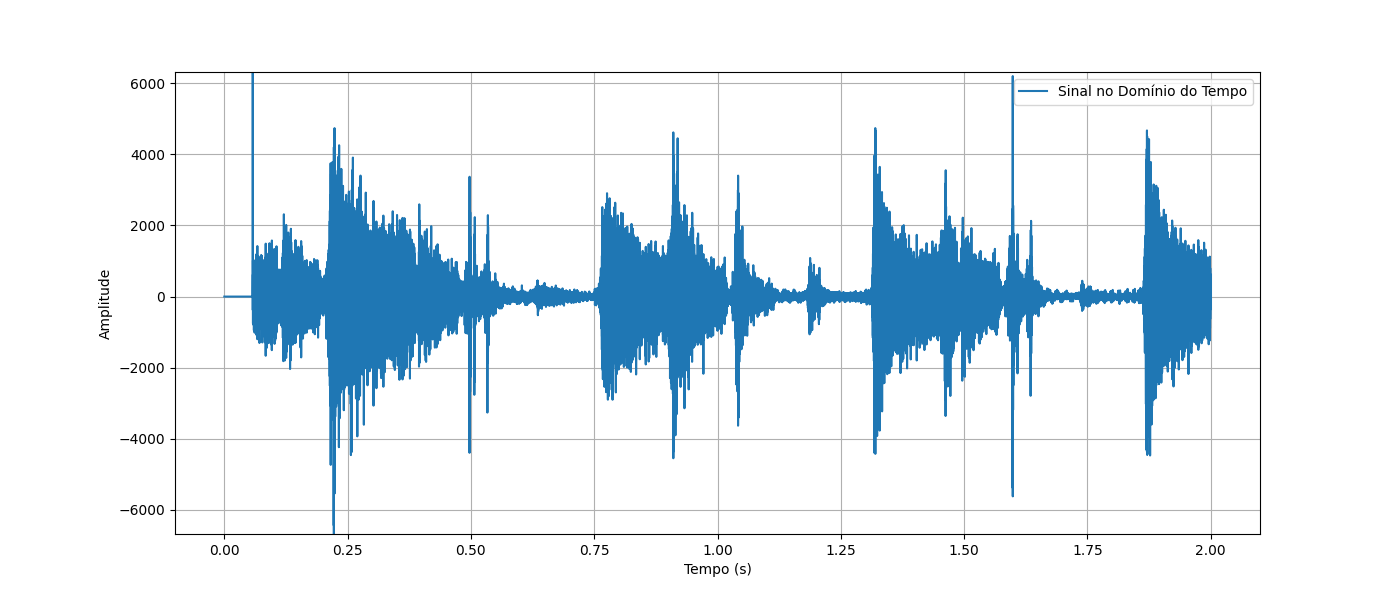
\includegraphics[width=0.8\textwidth]{figuras/fig68.png}
    \caption{canal de efeito \textit{reverb} isolado com música 1 a um volume de 0.6625}
    \label{fig68}
\end{figure}

A posição do botão central foi ajustada para observar a variação do volume do efeito. Na Figura \ref{fig68}, com a frequência de 9875 Hz, observou-se um volume maior.

\begin{figure}[h]
    \centering
    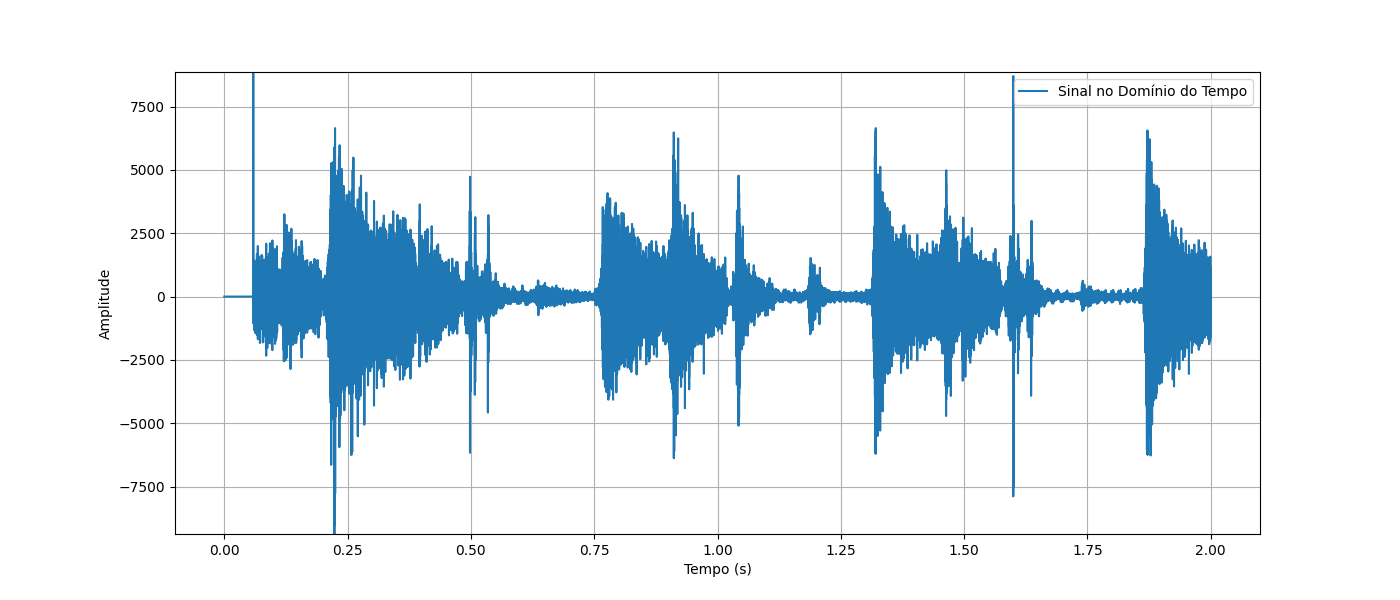
\includegraphics[width=0.8\textwidth]{figuras/fig69.png}
    \caption{canal de efeito \textit{reverb} isolado com música 1 a um volume de 1.0}
    \label{fig69}
\end{figure}
Para validar completamente a automação do volume, o botão central foi posicionado na frequência de 11025 Hz, que gera o volume máximo (1.0). A Figura \ref{fig69} mostra a ampliação do volume em função da variação da frequência, confirmando a automação do volume.

\subsection{\textit{Reverb}}

Para validar o controle do efeito de \textit{reverb}, o botão central foi posicionado para garantir que a frequência selecionada resultasse no volume máximo do efeito. Em seguida, ajustou-se a posição do botão de presença do efeito para observar a variação dos parâmetros. No caso do \textit{reverb}, a quantidade de dB presente após 1 segundo é configurada conforme o botão de parâmetro.

Nas figuras a seguir, são apresentadas representações do sinal no domínio do tempo, ilustrando a variação desse parâmetro. O intervalo de dB proposto no sistema varia de 0 a 1000 dB.


\begin{figure}[h]
    \centering
    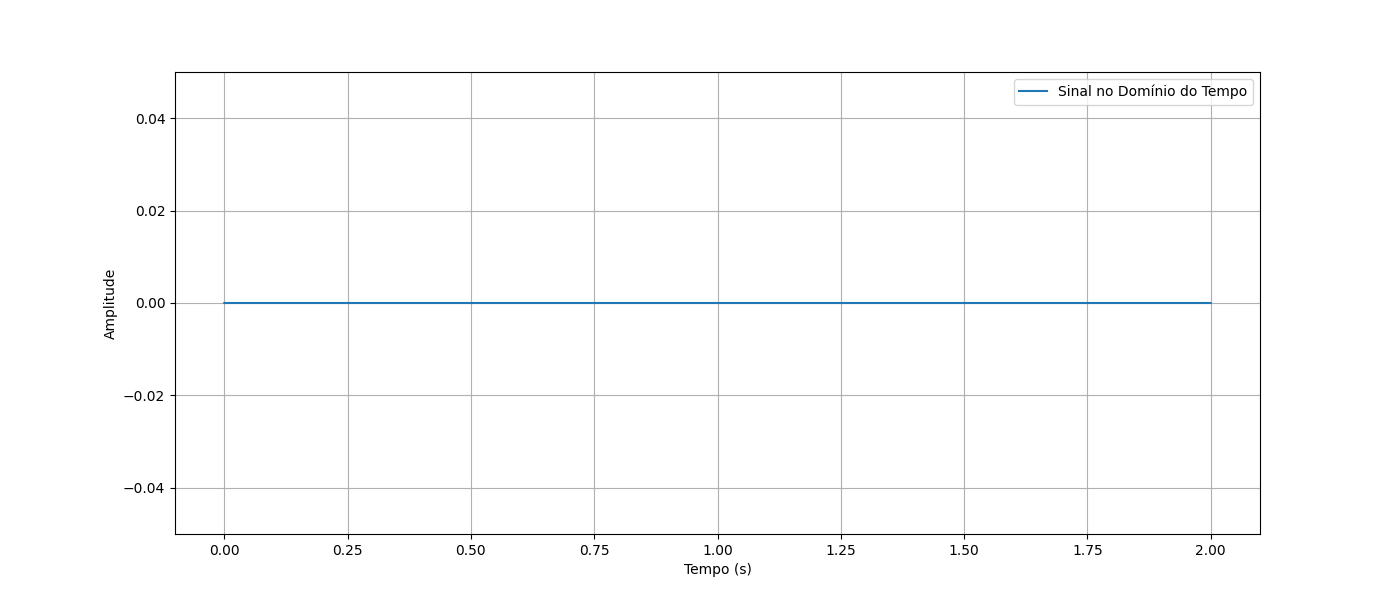
\includegraphics[width=0.8\textwidth]{figuras/fig70.png}
    \caption{\textit{reverb} com 0 dB após 1 segundo}
    \label{fig70}
\end{figure}

Na Figura \ref{fig70}, a posição inicial do botão de quantidade de efeito resulta em 0 dB após 1 segundo. Portanto, a forma de onda esperada também é nula, o que foi confirmado pelos resultados obtidos.

\begin{figure}[h]
    \centering
    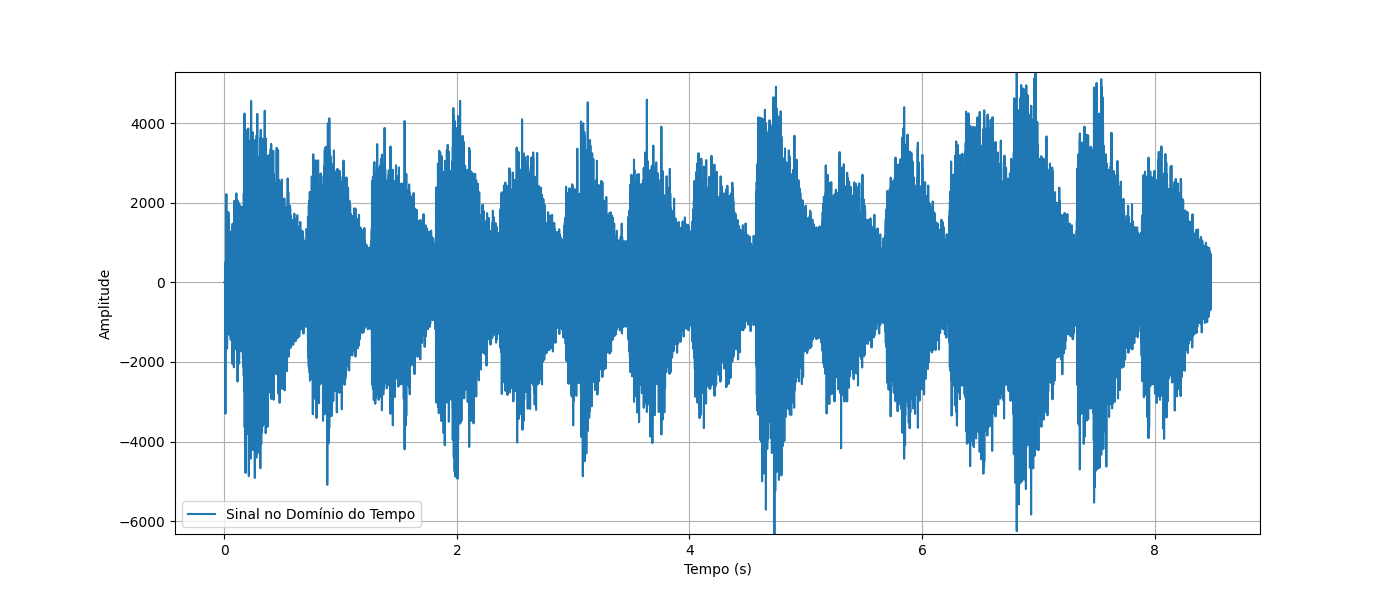
\includegraphics[width=0.8\textwidth]{figuras/fig71.png}
    \caption{\textit{reverb} com 25 dB após 1 segundo}
    \label{fig71}
\end{figure}

Em seguida, o botão de parâmetro de efeito foi ajustado para que 25 dB permanecessem após 1 segundo da amostra atual da música. Na Figura \ref{fig71}, observa-se a repetição de trechos da música devido à aplicação do efeito.


\newpage
\begin{figure}[h]
    \centering
    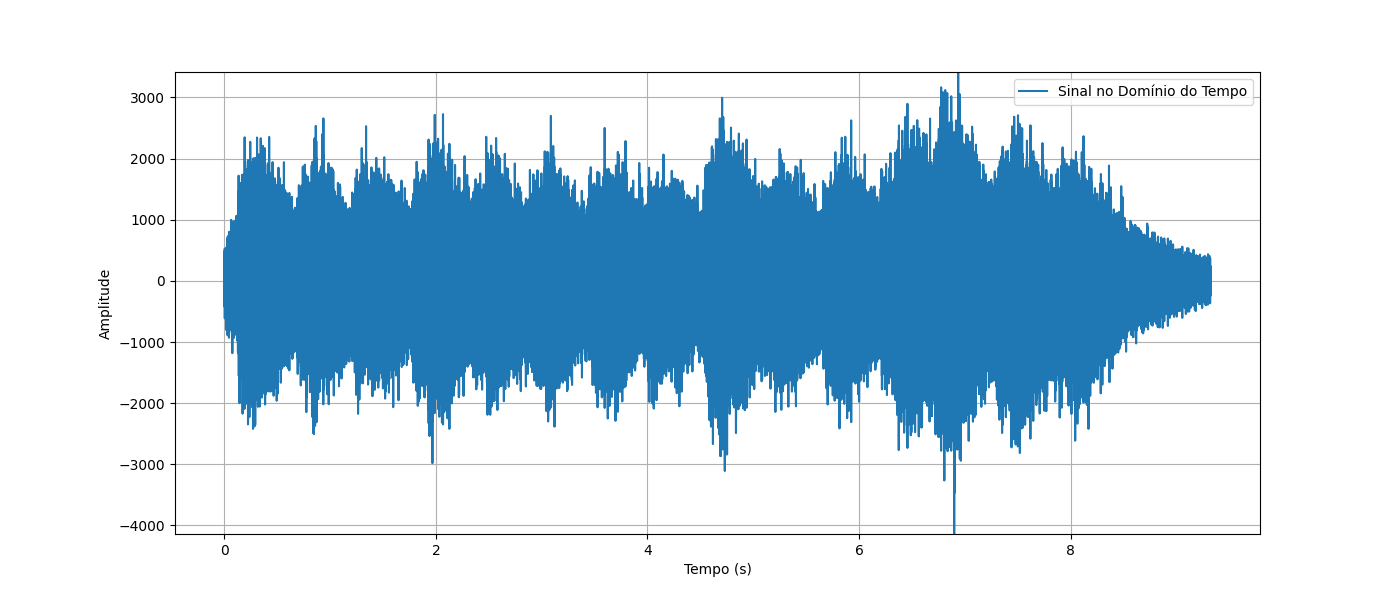
\includegraphics[width=0.8\textwidth]{figuras/fig72.png}
    \caption{\textit{reverb} com 50 dB após 1 segundo}
    \label{fig72}
\end{figure}

Com o aumento do ganho, o efeito de \textit{reverb} torna-se mais perceptível. Na Figura \ref{fig72}, é possível observar uma maior presença do efeito, com um aumento na amplitude do sinal ao longo do tempo.

\begin{figure}[h]
    \centering
    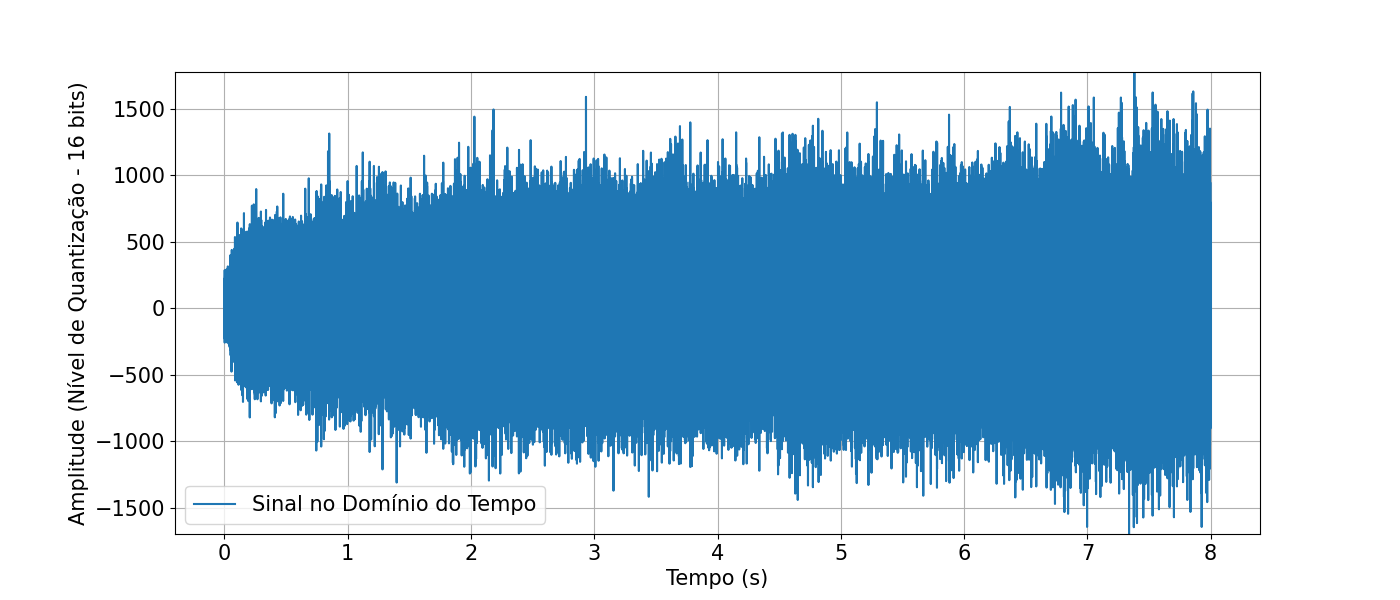
\includegraphics[width=0.8\textwidth]{figuras/fig73.png}
    \caption{\textit{reverb} com 100 dB após 1 segundo}
    \label{fig73}
\end{figure}

Finalmente, ao configurar 100 dB de ganho após 1 segundo, como mostrado na Figura \ref{fig73}, o efeito de \textit{reverb} é ainda mais pronunciado, resultando em um som com pouca definição. Isso indica que uma grande quantidade de som permaneceu, comprometendo a clareza da música.

\subsection{\textit{Delay}}

O efeito de \textit{delay} consiste em repetir o sinal após um determinado intervalo de tempo. As figuras a seguir ilustram o comportamento do efeito com diferentes configurações de atraso.

\newpage
\begin{figure}[h]
	\centering
    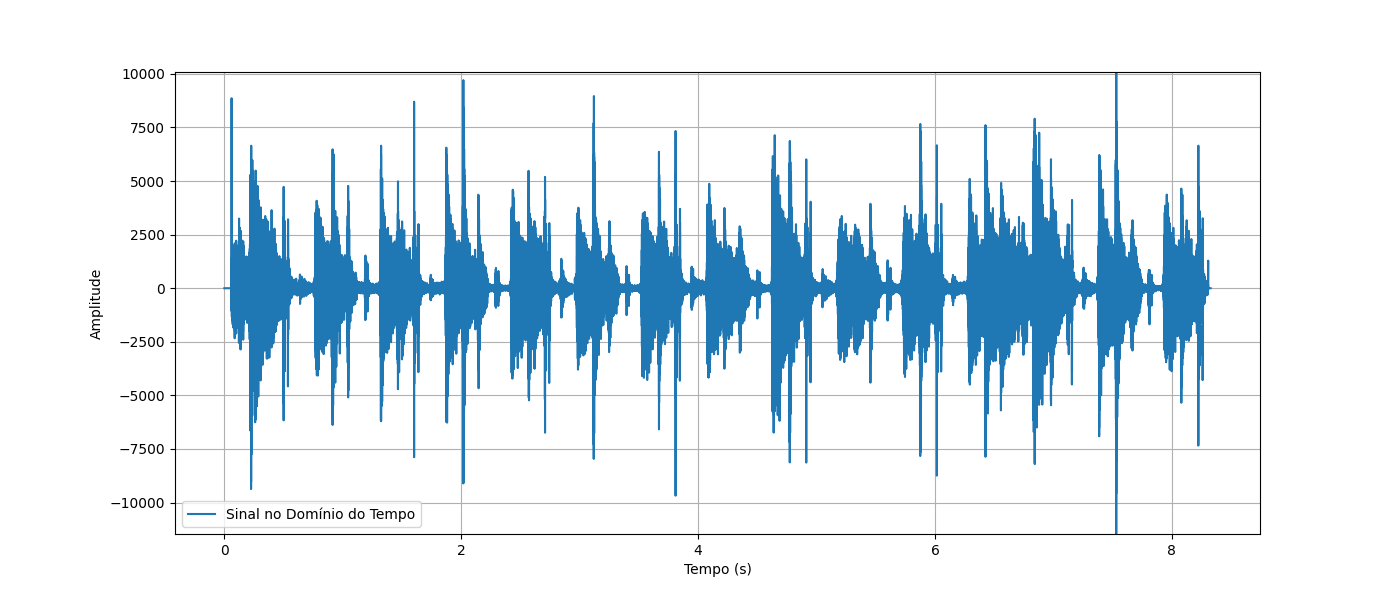
\includegraphics[width=0.7\textwidth]{figuras/fig74.png}
	\caption{\textit{delay} de 0 ms}
	\label{fig74}
\end{figure}

Na Figura \ref{fig74}, foi configurado um \textit{delay} de 0 ms. Nesse caso, a cópia do sinal é obtida imediatamente, sem atraso.

\begin{figure}[h]
	\centering
    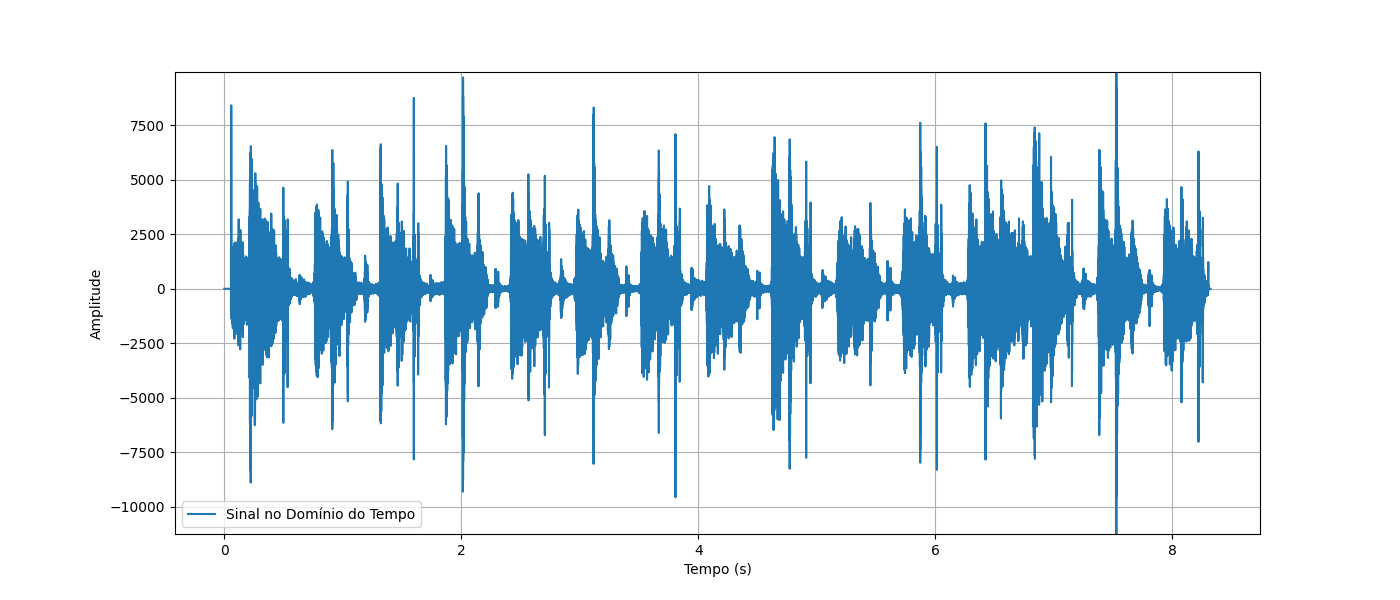
\includegraphics[width=0.7\textwidth]{figuras/fig75.png}
	\caption{\textit{delay} de 250 ms}
	\label{fig75}
\end{figure}

Na Figura \ref{fig75}, um \textit{delay} de 250 ms foi configurado. Aqui, a cópia do sinal é reproduzida com um atraso de 250 ms em relação ao sinal original.

\begin{figure}[h]
	\centering
    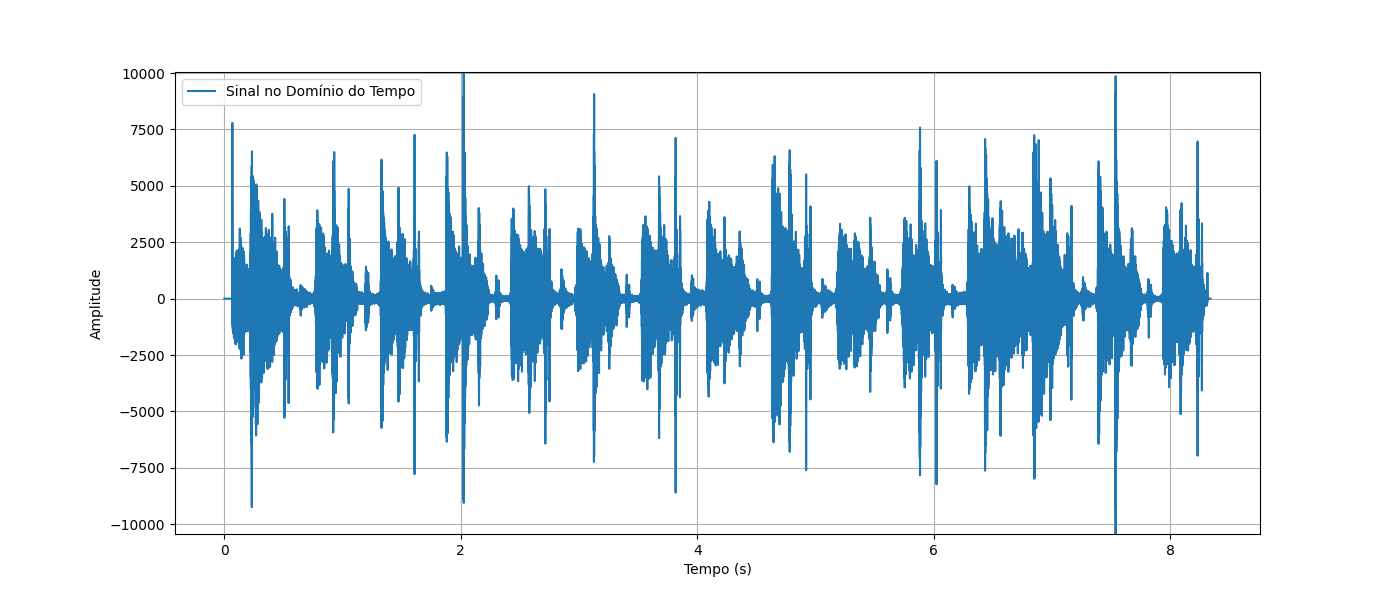
\includegraphics[width=0.7\textwidth]{figuras/fig76.png}
	\caption{\textit{delay} de 500 ms}
	\label{fig76}
\end{figure}

Na Figura \ref{fig76}, o \textit{delay} foi configurado para 500 ms. Neste caso, a cópia do sinal é reproduzida com um atraso de 500 ms em relação ao sinal original.

\newpage
\begin{figure}[h]
	\centering
    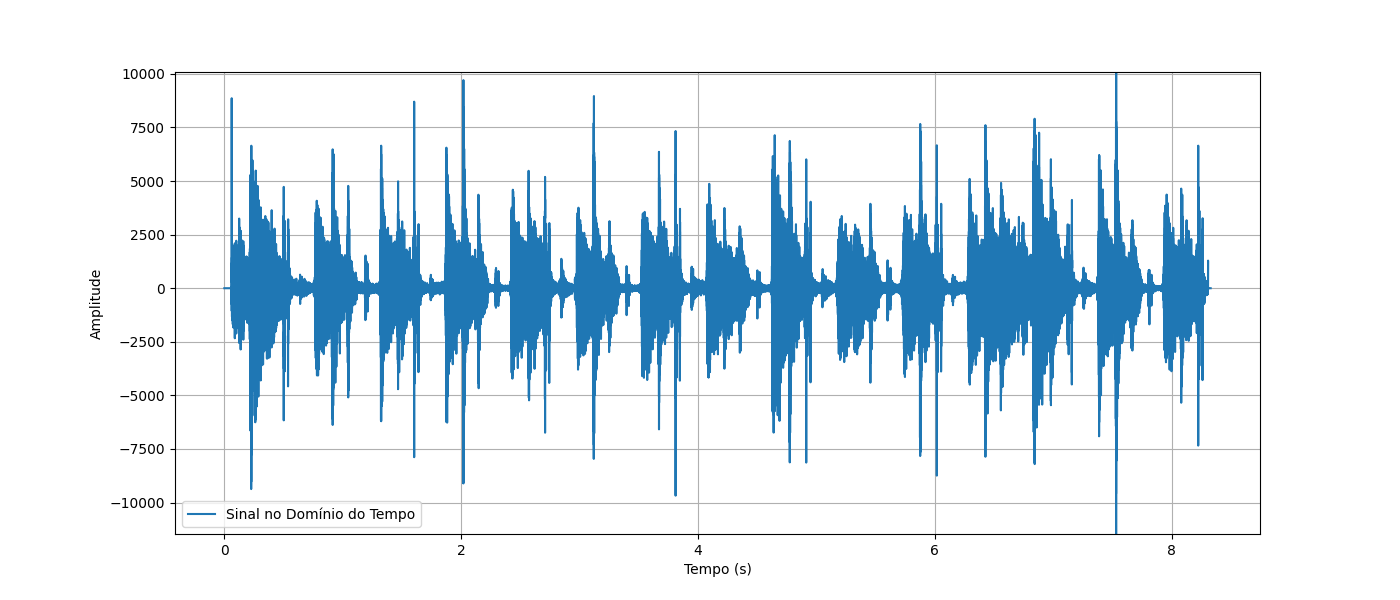
\includegraphics[width=0.7\textwidth]{figuras/fig77.png}
	\caption{\textit{delay} de 1000 ms}
	\label{fig77}
\end{figure}

Na Figura \ref{fig77}, foi configurado um \textit{delay} de 1000 ms. A cópia do sinal é reproduzida com um atraso de 1000 ms em relação ao sinal original.